\documentclass[a4,12pt]{article}

\usepackage[english]{babel}
\usepackage[utf8]{inputenc}
\usepackage[T1]{fontenc}
\usepackage[proportional]{libertine}
\usepackage[libertine]{newtxmath}

% Import the natbib package and sets a bibliography  and citation styles
\usepackage[numbers]{natbib}
\bibliographystyle{plainnat}
% \setcitestyle{numbers}

\usepackage{amsmath}
\usepackage{graphicx}
\usepackage{hyperref}
\usepackage{paralist}
\usepackage{xcolor}

%%% math
\newcommand{\betap}{\ensuremath{\beta^\prime}}
\newcommand{\data}{\ensuremath{\mathcal{D}}}
\newcommand{\expin}{\ensuremath{\lbrace\mu_i, \sigma_i\rbrace}}
\DeclareMathOperator{\Dirichlet}{Dirichlet}
\newcommand{\given}[2]{\left(#1\, \middle| #2 \, \right)}
\newcommand{\gaussian}{\ensuremath{\mathcal{N}}}
\newcommand{\genbetapr}{\ensuremath{\mathrm{GenBetaPrime}}}
\newcommand{\likelihood}{\ensuremath{\mathcal{L}}}
\newcommand{\lumi}{\ensuremath{\ell_i}}
\newcommand{\Lumi}{\ensuremath{L_i}}
\newcommand{\real}{\ensuremath{{\rm real}}}
\newcommand{\virt}{\ensuremath{{\rm virt}}}
\newcommand{\Nreal}{\ensuremath{N_\real}}
\newcommand{\Nvirt}{\ensuremath{N_\virt}}
\newcommand{\poisson}{\ensuremath{\mathrm{Poisson}}}
\newcommand{\rmdx}[1]{\mbox{d} #1 \,} % differential
\newcommand{\vecalpha}{\ensuremath{\vec{\alpha}}}
\newcommand{\vecL}{\ensuremath{\vec{L}}}
\newcommand{\vecmu}{\ensuremath{\vec{\mu}}}
\newcommand{\vecnu}{\ensuremath{\vec{\nu}}}
\newcommand{\vecth}{\ensuremath{{\vec{\theta}}}}
\newcommand{\vecu}{\ensuremath{{\vec{u}}}}

%%% refs
\def \refeq#1{(\ref{eq:#1})}
\def \refsec#1{sec.~\ref{#1}}
\def \refSec#1{Sec.~\ref{#1}}
\def \refapp#1{app.~\ref{#1}}
\def \reffig#1{fig.~\ref{fig:#1}}

%%% comments
\newcommand{\todo}[1]{{\textsc{\color{red}#1}}}

%%% codes
\newcommand{\tardis}{TARDIS}

\title{Formulating the posterior for \tardis}
\author{Frederik Beaujean}

\begin{document}
\maketitle

\section{Input and Output}

\subsubsection*{What we are given}
\begin{itemize}
\item data $\data \sim \expin =$ set of input values from
  telescope for each frequency bin $i=1 \dots n_b$;
\item \tardis{} depends on the parameters $\vecth$ and
  produces $n_\real$ real photon packets that leave the supernova and
  $n_\virt$ virtual photon packets. When we bin the packets in the same
  frequency bins as \expin, the sum of luminosities in bin $i$ is
  $\lumi^\real$ and $\lumi^\virt$.
\end{itemize}
I try to be mostly consistent with standard notation in statistics and
denote random variables---eventually they will be integrated out---by
capital letters and numbers that are observed by lower case.

\subsubsection*{What we want}
The posterior distribution of $\vecth$ given the data $\data$,
$P(\vecth | \data)$, is given by  Bayes' theorem as
\begin{equation}
  \label{eq:Bayes-full}
  P\given{\vecth}{\data} = \frac{P\given{\data}{\vecth} P(\vecth)}{\int \rmdx{\vecth} P\given{\data}{\vecth} P(\vecth)} \,.
\end{equation}
Technically, we should write every propability (density) as
conditional on a specific statistical model $M$,
e.g. $P\given{\vecth}{\data, M}$.  At present, we are not interested
in comparing different models but rather in extracting the parameters
of one model. Thus we omit $M$ and can ignore the denominator (the
\emph{evidence}) in Bayes' theorem. All we need is to define the
likelihood $\likelihood(\vecth) \equiv P\given{\data}{\vecth}$ and the
prior $P(\vecth)$ in
\begin{equation}
  \label{eq:Bayes-simple}
  P\given{\vecth}{\data} \propto \likelihood(\vecth) P(\vecth) \,.
\end{equation}

% Notation: $\vecth=$ parameters of interest,

% The overall goal is to extract (or maximize) the posterior of
% $\vecth$, the parameters that describe the physics behind
% supernovae. Bayes' theorem is
% \begin{align}
%   \label{eq:post}
%   P(\vecth | \mathcal{D}) &\propto P(\mathcal{D} | \vecth) P_0(\vecth)
% \end{align}
\section{Likelihood}

\subsubsection*{Goals}
\begin{itemize}
\item take into account uncertainty due to the finite number of packets in the simulation
\item model the distribution of luminosities accurately
\end{itemize}

\subsection{Incorporating the observations}

Let \Lumi{} denote the predicted or true luminosity in bin $i$ and
$\vecL$ the ordered collection of luminosities. I assume from a
telescope, we get the probability of the data $\mathcal{D}$ given
$\vecth$ only as a function of $\vecL$ where the data are
implicit---we don't have them---and no correlation between bins is
given or assumed. The maximum-entropy distribution given only the
means and standard deviations $\expin, i=1\dots n_b$ is the normal or
Gaussian distribution, so we set
\begin{equation}
  \label{eq:like-L}
  P(\mathcal{D} | \vecL) = \prod_{i=1}^{n_b} \gaussian\given{\Lumi}{\mu_i, \sigma_i^2}.
\end{equation}

In principle, $\vecL(\vecth)$ is a deterministic function of
$\vecth$. But we are unable to calculate it as is; that's why we have
to estimate it from the \tardis{} simulation resulting in a
distribution $P\given{\vecL}{\vecth}$. To use Bayes'
theorem~\refeq{Bayes-full}, we need $P\given{\data}{\vecth}$ but we
only have $P\given{\data}{\vecL}$. The link between these three
densities is the law of total probability:
\begin{align}
  \label{eq:like-expanded}
  P\given{\data}{\vecth} &= \int \rmdx{\vecL} P\given{\vecL}{\vecth} P\given{\data}{\vecL}.
\end{align}
Note that in principle it should say $P\given{\data}{\vecL, \vecth}$
in \refeq{like-expanded} but in our case $\vecth$ doesn't appear
explicitly, so we can just plug in
$P\given{\data}{\vecL}$ from~\refeq{like-L}.

\subsection{Extracting information from \tardis}

To complete the specification of the likelihood, we need to formulate
$P\given{\vecL}{\vecth}$; i.e., what we learn about the luminosities
in each bin from \tardis. A simplified account of how \tardis{} is run
follows, then I will show how to phrase this in statistical terms.

\subsubsection{Running \tardis}
\todo{This is still rudimentary}
\begin{compactenum}[(I)]
  \item Adjust the temperature of an inner shell to approximately match
    the total luminosity inferred from the observations
  \item Choose a total number of real packets, and a number of virtual
    packets to send out on each scattering of a real packet.
  \item Run \tardis.
  \item Some of the real packets reenter the core and are thus
    unobservable. But $n^\real$ real and $n^\virt$ virtual packets
    leave the core.
  \item Each packet has a luminosity. The packets are put into the
    same $n_b$ bins as the observations such that
    \begin{align}
      \label{eq:bin-packets}
      n^\real = \sum_{i=1}^{n_b} n_i^\real
    \end{align}
  \item The sum of real luminosities in bin $i$ is $\lumi^\real$.
\end{compactenum}
I usually omit the superscript $\in \{\real, \virt\}$ on $n_i$,
$\lumi$, and dependent quantities but equations hold for both unless
noted otherwise.

\subsubsection{Statistical model}

Some preliminary assumptions:
\begin{compactenum}[(a)]
  \item We neglect the uncertainty on the temperature and consider it
    fixed. We might lift this in the future.
  \item \label{assum:large-n} We neglect the uncertainty on $n^\real$ and consider it
    fixed. This should be a good approximation because we make sure
    $n^\real \gg 1$.
  \item \label{assum:large-nb} There are many bins; i.e., $n_b \gg 1$. So the probability of
    a packet to end up in any one bin is $\ll 1$.
\end{compactenum}
The proper distribution to describe the allocation of $n$ packets in
$n_b$ bins is the \emph{multinomial}. But in the limit of assumptions
(\ref{assum:large-n}) and (\ref{assum:large-nb}), we can consider the
Poisson distribution as a very good approximation. This in turn allows
us to consider the bins separately such that
\begin{align}
  \label{eq:factor-L}
  P\given{\vecL}{\vecth} = \prod_i P\given{L_i}{\vecth}
\end{align}
and the $n_b$-dimensional integral in \refeq{like-expanded}
dramatically simplifies to $n_b$ one-dimensional integrals.

The two major sources of statistical uncertainty coming from the
simulation are the unknown distribution of luminosity for the packets
and the Poisson uncertainty on the number of packets $n_i$. That is,
if we repeat the \tardis{} simulation with a different random-number
seed, we would get a different number of packets in bin $i$. The goal
in the following is to properly account for these two uncertainties
from a \emph{single} simulation without running repeatedly.

Let $N_i$ be the number of packets in we \emph{could} get in bin $i$
(it is not the number of packets we \emph{did} see, that's $n_i$),
then the law of total probability gives
\begin{equation}
  \label{eq:lum}
  P(\Lumi | \vecth) = \sum_{N_i=0}^{\infty} P(\Lumi | N_i, \vecth) P(N_i | \vecth)
\end{equation}
The first term in \refeq{lum} gives the luminosity in bin $i$ given
$N_i$ packets, so $\Lumi = \sum_{j=1}^{N_i} \Lumi^j$ where $\Lumi^j$ is
the luminosity of packet $j$ in bin $i$. Obviously $P(\Lumi | 0,
\vecth) = \delta(\Lumi)$.

We thought hard and found it a fair assumption that the distribution
of $l_{ij}$ is actually independent of the frequency thus independent
of $i$ and $j$ and we can drop the subscripts for simplicity, $l_{ij}
\to r$. The reason is that each packet initially gets the same
luminosity and so far it seems the amount of luminosity it gains or
loses is independent of the frequency. The question then is what is
the functional form $P(r | \vecth) \equiv P(\Lumi | N_i=1, \vecth)
$. The distributions $P(\Lumi | N_i, \vecth)$ with $N_i > 1$ can be
determined from the case of $N_i=1$ using convolutions for small $N_i$
and the central limit theorem for $N_i \ge 15$.

An approximation of $P(r | \vecth)$---a histogram of the luminosities
of all packets that leave the supernova---is shown in
\reffig{hist}.
\begin{figure*}[h]
  \begin{center}
    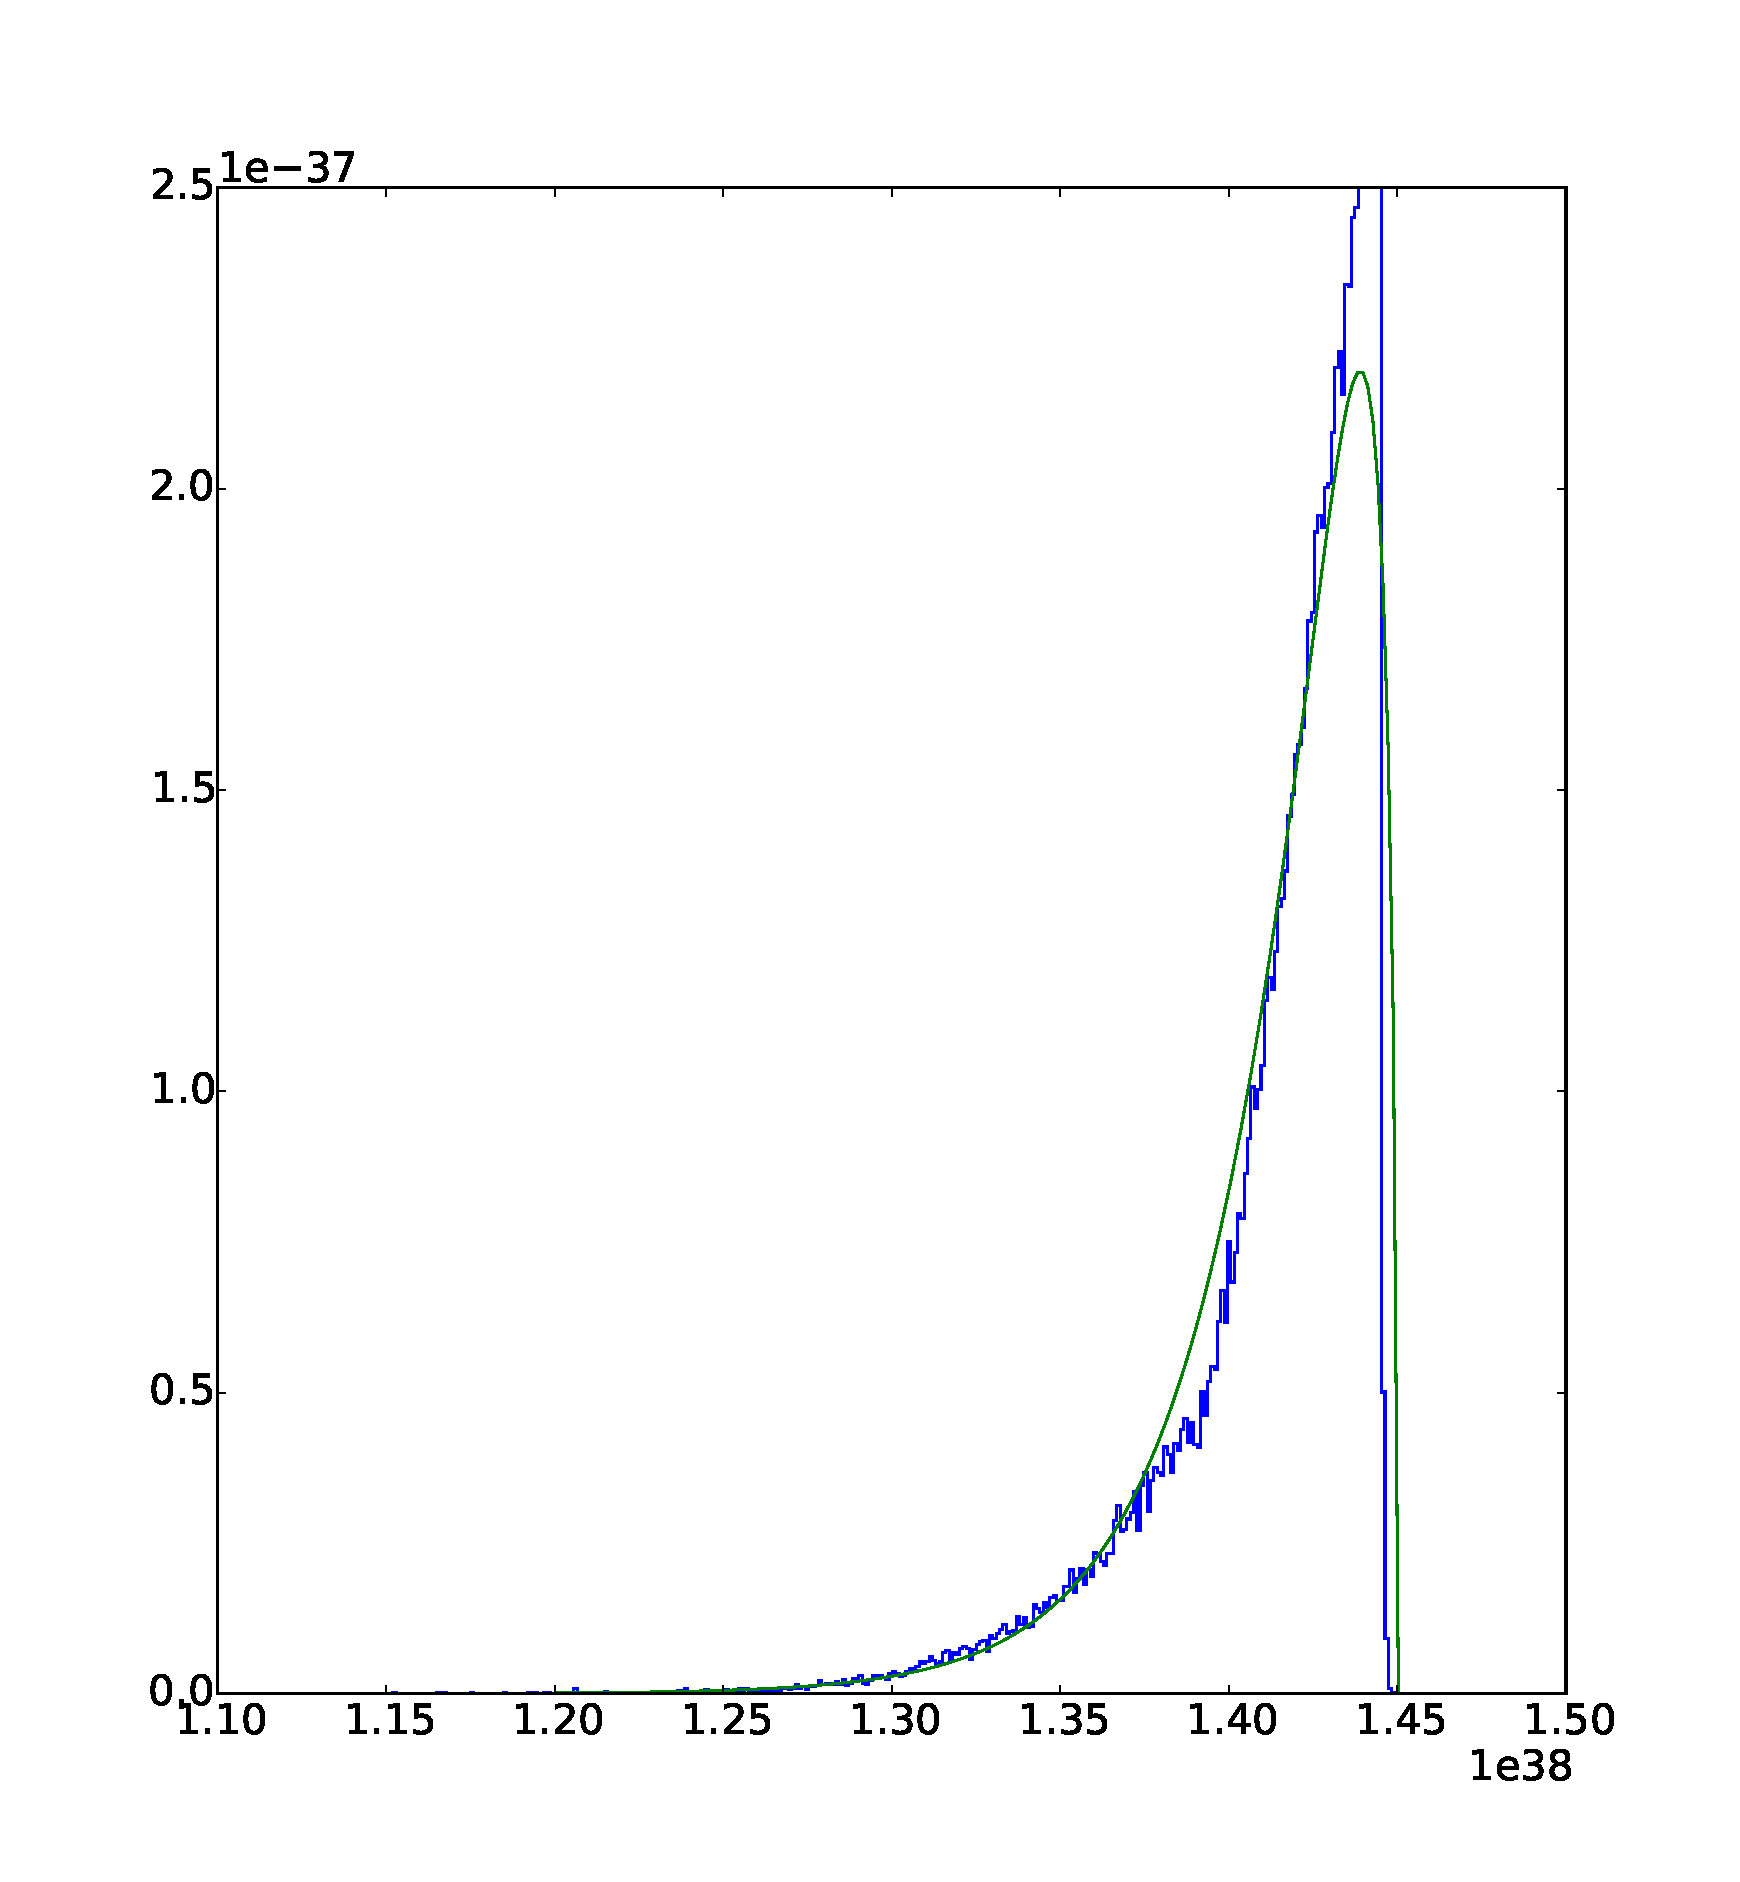
\includegraphics[width=\textwidth]{fit}
  \end{center}
  \caption{
  }
  \label{fig:hist}
\end{figure*}
The prominent features are a long tail at low luminosity, a sharp
peak, and a clear cutoff at high luminosity.  After researching quite
a bit, I found a flexible unimodal univariate distribution that can
accomodate this skewed distribution, it is the generalized \betap{}
distribution that depends on the hyperparameters $\vecnu \equiv (a, s,
\alpha, \gamma, \beta)$
\begin{equation}
  \label{eq:betaprime}
  P(r | \vecth) = \genbetapr(r | \vecnu(\vecth)) \equiv \frac{1}{B(\alpha, \gamma)} \left|\frac{\beta}{s} \right| \left( \frac{r - a}{s} \right)^{\alpha \beta - 1} \left(1+\left( \frac{r - a}{s} \right)^{\beta} \right)^{-\alpha - \gamma} \,.
\end{equation}

Since we assume it is the same in all bins we can then use the entire
set of samples that depend on $\vecth$ to infer $\vecnu | \vecth$. For
simplicity, we could use a maximum-likelihood fit and simply plug in
the result neglecting the uncertainty on $\vecnu$. This should be OK
as we usually have many packets; i.e., $N \gg 1$.

With $P(r|\vecth)$ fixed, we can now look at sums luminosities. The
standard result is that if $r_1, r_2 \sim P(r|\vecth)$ then
\begin{equation}
  \label{eq:convolution}
  z_2 = r_1 + r_2 \sim \int \rmdx{r} P(r|\vecth) P(z_2 - r|\vecth) \,.
\end{equation}
Sums of $N_i$ terms are computed in identical fashion by convolution
of $P(r|\vecth)$ with the distribution of the sum with $N_i-1$
terms. For $N_i \gtrsim 15$, the central limit theorem applies and
\begin{equation}
  \label{eq:clt}
  P(\Lumi | N_i, \vecth) \approx \gaussian \left(\Lumi | N_i * E_{P(r|\vecth)}[r], \sqrt{N_i * V_{P(r|\vecth)}[r]} \right)
\end{equation}
Note that for the convolutions, we would have to use the approximate
\genbetapr{} distribution but for the mean and std. deviation in
\refeq{clt}, we should use the sample mean and std. deviation to
bypass the extra uncertainty induced by assuming $P(r | \vecth) =
\genbetapr(r | \vecnu(\vecth))$ and fixed $\vecnu$.

For $P(N_i | \vecth)$, the second term in \eqref{eq:lum}, we assume
$N_i$ follows a Poisson distribution whose rate parameter $\lambda_i =
\lambda_i(\vecth)$ has to be inferred from the simulation. We can use
the law of total probability
\begin{equation}
  P(N_i | \vecth) = \int \rmdx{\lambda_i} P(\lambda_i | \vecth) \poisson(N_i | \lambda_i, \vecth)
\end{equation}
\todo{postpone the integral over $\lambda$ then use result for
  compound Poisson distr. and finally integrate. Hopefully this can
  still all be done analytically} and Bayes' theorem
\begin{equation}
  P(\lambda_i | \vecth) \propto \poisson(n_i | \lambda_i) P_0(\lambda_i)
\end{equation}
If we choose Jeffrey's prior $P_0(\lambda_i) \propto
1/\sqrt{\lambda_i}$ then we get the analytical
result~\cite[Eq. 5]{Aggarwal:2011aa}
\begin{equation}
  P\given{N_i}{n_i} = \frac{n_i! [2 (N_i + n_i)]!}{4^{N_i} N_i! (2 n_i)! (N_i + n_i)!}
\end{equation}
where $n_i = n_i(\vecth)$ is the number of packets in bin $i$ actually
observed in the simulation at hand.  In essence, $P(N_i | \vecth)$ is
the posterior predictive distribution to have $N_i$ packets given that
the simulation spit out $n_i(\vecth)$ packages. So $n_i$ is known,
while $N_i$ is a random variable and we take into account its
uncertainty by summing over $N_i$ in \refeq{lum}. This is relevant for bins where $n_i$ is small. If we got
2 packets, it is not so unlikely we could have gotten one package. But
of course with only half the packages, the expectation for the sum of
luminosities changes significantly.

\section{Priors}

\subsection{Polychord}

The polychord program only performs sampling and integration on the
unit hypercube with coordinates $\vecu$. Furthermore, it assumes that
the prior in these coordinates is uniform
\begin{equation}
  \label{eq:hypercube-prior}
  P(\vecu) = 1.
\end{equation}
In each iteration, we have to return the log likelihood for given
$\vecu$ passed in by polychord.  As above, suppose $\vecth$ represents
the parameters that are fed into the tardis simulation, then we need
to find the transform $\vecth(\vecu)$. The prior transforms as
\begin{equation}
  \label{eq:par-trafo}
  P(\vecth) \rmdx{\vecth} =  P(\vecu) \rmdx{\vecu},
\end{equation}
so with the flat prior
\begin{equation}
  \label{eq:par-trafo-likelihood}
  P(\vecth) = \left| \frac{\partial \theta_i}{\partial u_j} \right|^{-1} .
\end{equation}
There are two options:
\begin{enumerate}
\item \label{direct-transform} We can find $\vecth(\vecu)$ such that
  the Jacobian on the right in \refeq{par-trafo-likelihood} is the
  prior we want. The we just compute $\log L(\vecth(\vecu))$ for every
  sample $\vecu$ polychord provides.
\item If \ref{direct-transform} is not possible, we need to divide
  out the Jacobian and multiply by the actual prior we want, so for
  polychord we pretend we have a uniform prior and an \emph{effective} likelihood
  \begin{equation}
    \label{eq:eff-likelihood}
    L'(\vecu) = L(\vecth(\vecu)) P(\vecth(\vecu)) \left| \frac{\partial \theta_i}{\partial u_j} \right|
  \end{equation}
\end{enumerate}
Nested sampling is most efficient if the prior is close to the
posterior as measured by the relative entropy or Kullback-Leibler
divergence. \todo{cite Skilling} We therefore prefer
option~\ref{direct-transform}. While it restricts us to simple forms
of priors: uniform, Gaussian, or Dirichlet, this, fortunately, is
enough for our purposes. The explicit transformation is given below,
separately for each block of parameters.

% We could try to work out the
% transformation $\vecth(\vecu)$ such that the transformed prior has the
% form we want but for the relative abundances I don't know how to do
% that. Hence we will keep it simple and pretend that our prior is
% uniform and move everything into the effective likelihood $L'$. This
% amounts to perhaps slightly less efficient sampling but more
% importantly we can correctly define the target density from samples
% are produced. The Jacobian determinant can be computed as the product
% over blocks of correlated parameters.

\subsection{Relative abundances}

\subsubsection{Transformation}

Suppose we have $K$ abundances subject to the constraints
\begin{align}
  \label{eq:unit-simplex}
  & 0 \leq \theta_k \leq 1, & \sum_{k}\theta_k = 1.
\end{align}
In other words, the abundances are defined on the unit simplex.  As
shown in \todo{cite ``Cruising the simplex''}, we can directly
transform $\vecu$ with $\dim \vecu = K$ to $\vecth$ as follows. First
create $K$ Gamma variates with the inverse-transform method, in python
code $\xi_k = \texttt{scipy.stats.gamma.ppf}(u_k, \alpha_k)$ with the
shape parameter $\alpha_k$ explained below. Then normalize the samples
as
\begin{equation}
  \label{eq:dirichlet-gamma}
  \theta_k = \frac{\xi_k}{\sum_{k'} \xi_{k'}}.
\end{equation}
such that
\begin{equation}
  \label{eq:dirichlet-prior}
  P(\vecth) = \Dirichlet(\vecth | \alpha)
\end{equation}

\subsubsection{Prior information}

The canonical choice of a prior for fractions such as relative
abundances is the Dirichlet
distribution~\cite[App.~B]{bishop_pattern_2006}
\begin{equation}
  \label{eq:dirichlet-def}
  \Dirichlet \given{\vecth}{\vecalpha} = \frac{\Gamma\left(\sum_k \alpha_k\right)}{\prod_k \Gamma(\alpha_k)} \prod_{k=1}^K \theta_k^{\alpha_k-1}
\end{equation}
and depends on $K$ parameters $\vecalpha$. How to choose $\alpha_k$?
The mode of $\theta_k$ is $\frac{\alpha_k - 1}{\sum_k (\alpha_k -
  1)}$, so we should choose $\alpha_k > 1$ if we want a well defined
mode. For prior ignorance, we want $\alpha_k$ identical. The canonical
choice of an uninformative distribution is a uniform distribution on
the unit simplex given by $\alpha_k=1 \, \forall \, k$~\todo{cite
  posterior predictive hints}.

Now suppose we want to include the available prior information. The
actual numbers come from table 5.1 of Wolfgang's thesis. He lists
constraints of the type
\begin{equation}
  \begin{aligned}[t]
    \label{eq:abundance-constraints}
    \mbox{C}  &< 12.5 \%,\\
    \mbox{Si} &>1 \%,\\
    1 &<\mbox{Si/S ratio} < 10 .
  \end{aligned}
\end{equation}
The most straightforward approach is to incorporate them as hard cuts
into the prior, leading to a new normalization. We will have to refine
this strategy if the regions of high posterior probability turn out to
be very close to the cuts. Formally, suppose $V$ is the subvolume of
the unit simplex in which all constraints are satistfied. Outside of
$V$, we set $P(\vecth) \equiv 0$. In the code, a sequence of
\texttt{if} statements incorporates the constraints. If any is
violated, the prior on the log scale is $-\infty$ and no tardis
simulation needs to be run. Our prior thus becomes
\begin{equation}
  \label{eq:abundances-prior}
  P(\vecth) = C_V^{-1} \mathbf{1}_V(\vecth) \Dirichlet\left(\vecmu(\vecth) \middle| \vecalpha=(10^{-4}, \dots, 10^{-4})\right) \boldsymbol{\theta}
\end{equation}
where the normalization constant $C_V$ is  determined from
\begin{equation}
  \begin{aligned}
    \label{eq:abundance-normalization}
    1 &= \int \rmdx{\vecth} P(\vecth)\\
    \Rightarrow C_V  &= \int_V \rmdx{\vecth} \Dirichlet\left(\vecmu(\vecth) \middle| \vecalpha=(10^{-4}, \dots, 10^{-4})\right)
  \end{aligned}
\end{equation}
and $\mathbf{1}_V$ is the indicator function on $V$; i.e.,
$\mathbf{1}_V(\vecth) = 1$ iff $\vecth \in V$.  If we keep the cuts
fixed, we only need to determine $C_V$ once. We can do that with good
precision without nested sampling by using the law of large numbers as
\begin{equation}
  \label{eq:abundances-large-numbers}
  C_V \approx \frac{1}{N} \sum_{i=1}^N \mathbf{1}_V(\vecth), \; \vecth \sim \Dirichlet\left(\vecmu(\vecth) \middle| \vecalpha=(10^{-4}, \dots, 10^{-4})\right)
\end{equation}
and drawing directly from $\Dirichlet(\vecalpha)$ using
\texttt{scipy.random.dirichlet}. However, we don't really need to
normalize our densities properly unless we compare different
models. In the near future, we will only infer the parameters of a
single model so there is no need to compute $C_V$.

\subsection{Other parameters}

For all parameters other than abundances we choose uniform priors to
start with. This is not necessarily noninformative but we should be a
proxy for a diffuse prior hoping that the likelihood is sharp enough
to constrain all parameters. In the end, we should study the prior
dependence by choosing some other distribution such as wide Gaussians
or Cauchys to see if it has a significant effect.

\bibliography{references}

\end{document}
